

%\documentclass[conference]{IEEEtran}
%\IEEEoverridecommandlockouts
\documentclass{article}  
\twocolumn

\usepackage{graphicx}
\usepackage{algorithm}
\usepackage{algorithmic}
\usepackage{amsmath}
\usepackage{adjustbox}
\usepackage{authblk}
\usepackage{pbox}
\usepackage{float}
\usepackage[margin=1in]{geometry}
\author[1]{Dalia Ibrahim}
\author[2]{Carlos Dasaed Salcedo}


{
    \makeatletter
    \renewcommand\AB@affilsepx{: \protect\Affilfont}
    \makeatother
        
        

    \affil[ ]{Studnet ID}

    \makeatletter
    \renewcommand\AB@affilsepx{, \protect\Affilfont}
    \makeatother

    \affil[1]{201893217}
    \affil[2]{201892008}
    
        \makeatletter
\setlength{\floatsep}{5pt}
\setlength{\textfloatsep}{5pt}
    \makeatother
    
}

\begin{document}  

\title{ Assignment 4: Recognizing  House Numbers with Deep Neural Network }


\maketitle
 \section{Introduction}

For this assignment, we have implemented a program that takes as input a training data set and a testing dataset from the SVHN samples in .mat format, creates a deep convolutional neural network, and saves a trained model as Model.h5. We used SciKit Learn libraries, numpy, pandas, matplotlib, h5py, and the Keras functional API from Tensorflow to generate the trained a Deep  Convolutional Neural Network(DCNN) model. To test and validate the model, several different types of layers were tested until an accuracy of 90% was achieved. 


\section{Data Pre-processing}
The primary task at hand was to classify house numbers given in pictures, which makes the colours of the image almost irrelevant as a red five or a blue five would still be classified as a 5. Based on this reasoning, we decided to convert all the training and testing data sets to grey scale. This drastically reduces the initial input of the DCNN as we deal with with a single value per pixel, rather than the three values obtained from the RGB format. Since the colours of each pixel will always range from 0 to 255, we decided to apply a simple normalization step by dividing the value of each pixel by 255. This way, all pixels will now have a value between 0 and 1.

\section{MODEL PARAMETERS}

The model parameters were all selected and tested by hand, as there is not an efficient method for selecting the number of layers, type of layers, activation functions, amongst other features, other than by trial and error. We started with the default values of the examples found in the Tensorflow documentation, and then proceeded to modify various parameters. Since the program was being executed locally in our computers, we did not have the computational power of servers generally used for this kind of tests as that of IBM’s Watson, or Google’s Alpha Go projects. 

\begin{itemize}

  \item{Activation Function} Two activation functions were tested: ReLU and Sigmoid. ReLU is generally considered to a good default function for any ML model, and hence, was the first function we decided to test. For testing purposes, we selected Sigmoid, as we wanted to compare the performance   different activation functions. Ultimately, the ReLU function proved to be faster and yielded more accurate results than the Sigmoid function.
  
   \item{  Optimizer}
   The first optimizer tested was ADAM. Since we are more familiar with stochastic gradient descent, we also tested SGD, and obtained  WORSE results in both, accuracy of the model and training time. Our final selection was ADAM.
   
     \item{ Number of epochs and batch size}
     Although, in the literature and in tutorials, values ranging from 10 to extremely large numbers may be selected,  we decided to use an epoch value of 10, as our computational power was limited, and we wanted to avoid overfitting. Likewise, our batch parameter was set to 100 to keep our running as low as possible without compromising too much on accuracy.
     
      \item{Metrics}
   For this assignment, we only focused on accuracy, rather than the AUPRC which was used in previous assignments, since our goal was on obtaining the most accurate model possible from the given training samples. 
    \item{ Regularization}
    In an effort to reduce the generalization error, we have used the dropout function offered in the Keras library. 
\end{itemize}
\section{RESULTS}
    We have created a table containing the parameters modified and the accuracy obtain from the various tests that were done with the code


\begin{figure}[h]
  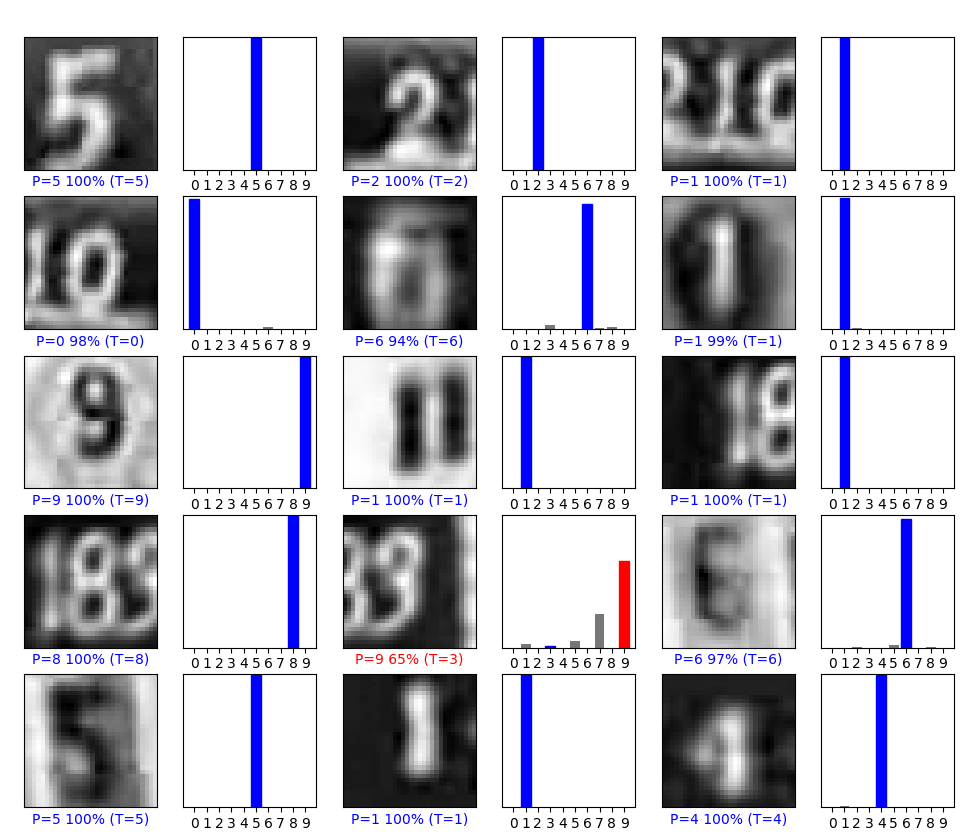
\includegraphics[width=\textwidth]{results.png}
  \caption{This is a tiger.}
\end{figure}

\pagebreak
\newpage
\clearpage

\begin{adjustbox}{angle=90}
%\begin{table}[]
%\begin{tabular}{|l|l|l|l|l|l|}
\begin{tabular}{|p{2cm}|p{3cm}|p{3cm}|p{3cm}|p{3cm}|p{3cm}|}
\hline
\textbf{}&\textbf{Architecture 1} & \textbf{Architecture 2}                                             & \textbf{Architecture 3}                       & \textbf{Architecture 4}                                    & \textbf{Architecture 5}                                                                                         \\ \hline
                        & CNN  32 hiden unitsActivation function = RELUKernel\_ size ( 3 X 3) & CNN  32 hiden unitsActivation function = RELU & CNN  32 hiden unitsActivation function = RELUAllowPadding  & CNN  32 hiden unitsActivation function = RELUAllowPadding  & CNN  32 hiden unitsActivation function = SigmoidAllowPadding  \\ \hline
                        & CNN  64 hiden unitsActivation function = RELU                       & CNN  64 hiden unitsActivation function = RELU & CNN  64 hiden unitsActivation function = RELU AllowPadding & CNN  64 hiden unitsActivation function = RELU AllowPadding & CNN  64 hiden unitsActivation function = Sigmoid AllowPadding \\ \hline
                        & Max pooling size ( 2 x 2)                                           & CNN  64 hiden unitsActivation function = RELU & CNN  64 hiden unitsActivation function = RELUAllowPadding  & CNN  64 hiden unitsActivation function = RELUAllowPadding  & CNN  64 hiden unitsActivation function = SigmoidAllowPadding  \\ \hline
                        & Dropout ( 0.25)                                                     & CNN  64 hiden unitsActivation function = RELU & CNN  64 hiden unitsActivation function = RELUAllowPadding  & CNN  64 hiden unitsActivation function = RELUAllowPadding  & CNN  64 hiden unitsActivation function = SigmoidAllowPadding  \\ \hline
                        & Flatten                                                             & Max pooling size ( 2 x 2)                     & Max pooling size ( 2 x 2)                                  & Max pooling size ( 2 x 2)                                  & Max pooling size ( 2 x 2)                                     \\ \hline
                        & Dense128 Hidden units Activation = RELU                             & Dropout ( 0.25)                               & Dropout ( 0.25)                                            & Dropout ( 0.25)                                            & Dropout ( 0.25)                                               \\ \hline
                        & Dropout ( 0.25)                                                     & Flatten                                       & Flatten                                                    & Flatten                                                    & Flatten                                                       \\ \hline
                        & Dense10 Hidden units Activation = Softmax                           & Dense128 Hidden units Activation = RELU       & Dense128 Hidden units Activation = RELU                    & Dense128 Hidden units Activation = RELU                    & Dense128 Hidden units Activation = Sigmoid                    \\ \hline
                        &                                                                     & Dense10 Hidden units Activation = Softmax     & Dense10 Hidden units Activation = Softmax                  & Dense10 Hidden units Activation = Softmax                  & Dense10 Hidden units Activation = Softmax                     \\ \hline
\textbf{optimizer}      & adam                                                                & adam                                          & adam                                                       & \textbf{SGD}                                               & adam                                                          \\ \hline
\textbf{loss Function}  & categorical \_crossentrop                                            & categorical \_crossentrop                      & categorical \_crossentrop                                   & categorical \_crossentrop                                   & categorical \_crossentrop                                      \\ \hline
\textbf{Accuracy}       & 87.00\%                                                             & 90.00\%                                       & 90.00\%                                                    & 88.00\%                                                    & 60.00\%                                                       \\ \hline
\end{tabular}
%\end{table}
\end{adjustbox}




\end{document}